\documentclass[conference]{IEEEtran}
\IEEEoverridecommandlockouts
% The preceding line is only needed to identify funding in the first footnote. If that is unneeded, please comment it out.
\usepackage{cite}
\usepackage{amsmath,amssymb,amsfonts}
\usepackage{algorithmic}
\usepackage{graphicx}
\usepackage{textcomp}
\usepackage{xcolor}
\usepackage{hyperref}
\usepackage{chemmacros}
\def\BibTeX{{\rm B\kern-.05em{\sc i\kern-.025em b}\kern-.08em
    T\kern-.1667em\lower.7ex\hbox{E}\kern-.125emX}}
\renewcommand\IEEEkeywordsname{Keywords}

\begin{document}

\title{ Implementation of Grover’s Algorithm based on
	Quantum Reservoir Computing  \\

}
\author{
	\IEEEauthorblockN{Jyothikrishna Sajja}
	\IEEEauthorblockA{\textit{Department of ECE,} \\
		\textit{IIITDM Kancheepuram,}\\
		Chennai-600127, India. \\
		ec21b1022@iiitdm.ac.in}
	\and
	\IEEEauthorblockN{Vikrant Abhishek}
	\IEEEauthorblockA{\textit{Department of ECE,} \\
		\textit{IIITDM Kancheepuram,}\\
		Chennai-600127, India. \\
		ec21b1116@iiitdm.ac.in}
	\and
	\IEEEauthorblockN{Shivani Mehta}
	\IEEEauthorblockA{\textit{Department of ECE,} \\
		\textit{IIITDM Kancheepuram,}\\
		Chennai-600127, India.\\
		ec22m2002@iiitdm.ac.in}
	\and

	\IEEEauthorblockN{Sumanth Arige}
	\IEEEauthorblockA{\textit{Department of ECE,} \\
		\textit{IIITDM Kancheepuram,}\\
		Chennai-600127, India. \\
		edm20d010@iiitdm.ac.in}
	\and

	\IEEEauthorblockN{V.Praveen Bhallamudi}
	\IEEEauthorblockA{\textit{Department of Physics,} \\
		\textit{IIT Madras,}\\
		Chennai-600036, India. \\
		praveen.bhallamudi@iitm.ac.in}
	\and

	\IEEEauthorblockN{ Tejendra Dixit, $Member, IEEE$}
	\IEEEauthorblockA{\textit{Department of ECE,} \\
		\textit{IIITDM Kancheepuram,}\\
		Chennai-600127, India. \\
		tdixit@iiitdm.ac.in}
}

\maketitle

\begin{abstract}
	Quantum computing represents the leading edge of
	computational technology, leveraging the principles of quantum
	mechanics to execute targeted computations much faster than
	classical computers. In contrast to classical bits, which are limited
	to representing either 0 or 1, qubits, or quantum bits, exhibit
	the extraordinary property of superposition. This distinctive
	characteristic enables qubits to simultaneously occupy multiple
	states, empowering quantum computers to explore numerous
	potential solutions to a problem concurrently. This feature
	makes quantum computing particularly potent for specific tasks.
	Recent research endeavors have been sparked by the potential
	of advanced quantum computing technology, leading to the
	creation of simulations of quantum computers using classical
	hardware. Grover’s quantum search algorithm serves as a notable
	illustration of quantum computing application, enabling quantum
	computers to conduct a database search within an unsorted array
	with a quadratic speedup in time efficiency compared to classical
	computers. This document presents the quantum Grover search
	algorithm and its application through 5-qubit quantum circuits,
	as well as a design framework to simplify the creation of an
	oracle for a greater number of qubits.
\end{abstract}

\begin{IEEEkeywords}
	Quantum computation, Qubits, Oracle, Grover’s
	algorithm, IBM Qiskit.
\end{IEEEkeywords}

\section{Introduction}
% Discuss quantum computing and grover's algorithm.
Quantum computing is a new frontier in computer science that utilises the unique phenomena of quantum physics to solve problems that are too complex for classical computers to handle.\cite{b0}. Quantum computing algorithms are specialised procedures designed to harness the unique capabilities of quantum computers to solve problems more efficiently than classical algorithms. These algorithms leverage quantum phenomena like superposition and entanglement to explore multiple possibilities simultaneously, leading to potential speedups for certain types of tasks. One such algorithm is Grover's algorithm\cite{b1}. With Grover's algorithm searching an unsorted database is quadratically faster than classical algorithms.
\\
% Discuss what has been done till now.
Grover's algorithm has been implemented on publicly available quantum computers like IBM Q 5 Tenerife (5-qubit chip) and IBM Q 16 Rüschlikon (16-qubit chip) \cite{b2} and on programmable quantum computer consisting of a
linear chain of five trapped ions \cite{b3} . While the early implementations were on small-scale devices with limited qubits, significant progress has been made in recent years.

% Discuss what we will be doing.
Our goal is to investigate the readiness of current IBM quantum computers to support the execution of Grover's algorithm.

\section{Background and Methodology}

The Grover search algorithm, conceived by Lov Grover
in 1996, stands as a quantum computing method offering
a quadratic acceleration compared to classical counterparts,
particularly for solving unstructured search problems [8]. It
has gained renown for its proficiency in searching through
unsorted databases, but its utility extends to a spectrum
of tasks, encompassing cryptographic problem-solving and
quantum system simulation. This can speed up a search
problem quadratically. For N number of unsorted data classical
computer require O (N) operations Whereas Grover is optimal
and can do this in O($ \sqrt{N} $) operation. The following provides
a synopsis of the workings of the Grover search algorithm [9]:
\subsection{Initialisation}
Commencing the process involves establishing a superposition of all conceivable states. For instance, when seeking an
item in a database housing N item, quantum parallelism is
harnessed to generate a superposition of all N states as shown
in Fig.1. Achieving this involves a sequence of quantum gate
operations.

\begin{figure}[htbp]
	\centerline{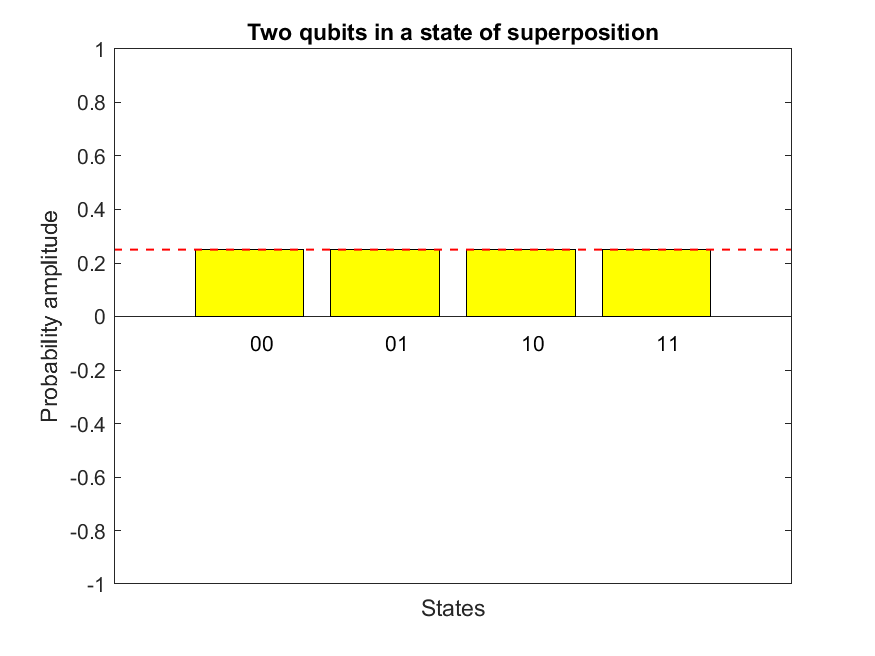
\includegraphics[width=9cm,height=10cm,keepaspectratio]{fig1.png}}
	\caption{Superposition of 2 qubits}
	\label{fig1}
\end{figure}

\subsection{Oracle Function}
Grover’s algorithm hinges on the application of an oracle
function, often denoted as \textbf{"$ U_f $"}. This oracle acts to mark
the target state(s) by inverting their sign. For instance, if the
objective is to locate a specific item in a database, the oracle
would negate the amplitude corresponding to the target item.
In Fig. 2, it is graphically shown the oracle function flipping
the correct target.

\begin{figure}[htbp]
	\centerline{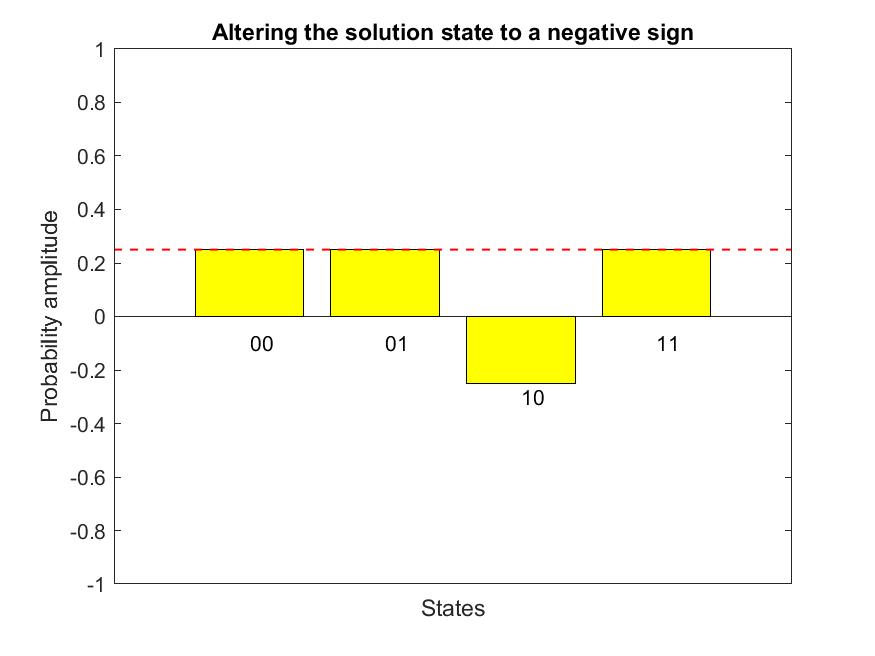
\includegraphics[width=9cm,height=10cm,keepaspectratio]{fig2.png}}
	\caption{Altering the sign of solution state(10)}
	\label{fig2}
\end{figure}

\subsection{Amplitude Amplification}
The core of the Grover algorithm is the process of amplitude
amplification, which entails two central maneuvers:
\begin{itemize}
	\item \textbf{Inversion around the Mean}: During this stage, the amplitudes are mirrored around their average value, thus  boosting the amplitude of the desired state(s) while reducing the amplitudes of the non-desired states.
	\item \textbf{Grover diffusion operator}: In this step, the amplitudes
	      of the target state(s) are further augmented through the
	      application of a suite of quantum gates [10].

\end{itemize}
After acting of Grover diffusion operator, the final output will
have amplified magnitude as shown in Fig. 3.
\subsection{Reiteration}
Step. 2 and step. 3 are iterated approximately $ \sqrt{N} $ times
to maximize the likelihood of detecting the correct state. This
number of iterations ensures that the probability of identifying
the correct state approaches near certainty.

\begin{figure}[htbp]
	\centerline{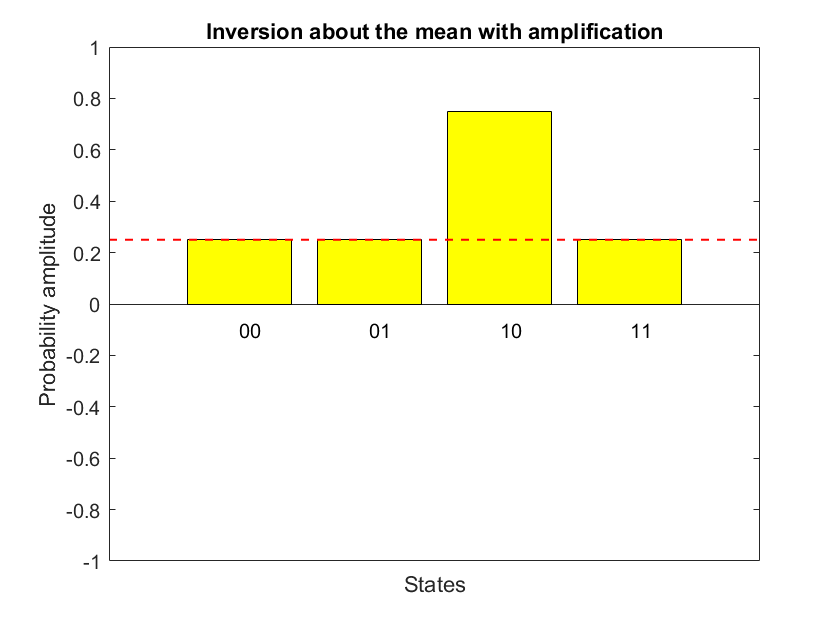
\includegraphics[width=9cm,height=10cm,keepaspectratio]{fig3.png}}
	\caption{Inversion about the mean with amplification.}
	\label{fig3}
\end{figure}

\subsection{ Measurement}
Ultimately, the quantum state is subjected to measurement.
The target state is discerned with notably higher probability in comparison to the non-target state.

\section{ CONSTRUCTION OF ORACLE AND DIFFUSION
  OPERATOR}
The Grover iteration, also known as the Grover operator,
constitutes a crucial component of the quantum search process.
It encompasses two distinct phases. At the outset, the oracle
function modifies the phase of a single amplitude within a
marked state. Upon completion of this phase, referred to as
the diffusion layer, the indicated state amplitude is flipped.
Consequently, while the amplitudes of the other states remain
unchanged, the target state assumes an inverted state, resulting
in a notable increase in its amplitude and a slight decrease in
the amplitudes of the other states. The block diagram of Grover
iteration circuit is shown below in Fig. 4.

\begin{figure}[htbp]
	\centerline{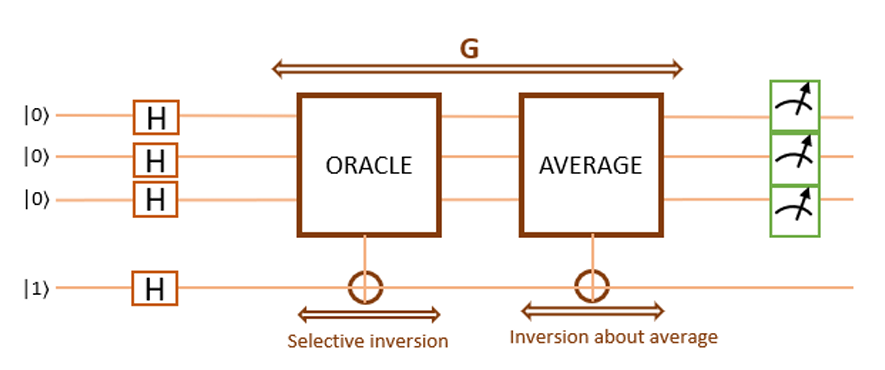
\includegraphics[width=9cm,height=10cm,keepaspectratio]{fig4.png}}
	\caption{Grover Iteration circuit}
	\label{fig4}
\end{figure}

\subsection{Oracle}
In
quantum computing, a quantum oracle [11] is a computational
component that furnishes data pertinent to the particular prob
lem or task undergoing processing by the quantum algorithm.
The quantum oracle performs a bit-flip on the oracle qubit when the input corresponds to a valid solution. Oracle can be understood as described below.

$ Oracle(x) = (-1)^{f(x)} |x \rangle $

$ f(t) = \begin{cases}
		1, & t = x     \\
		0, & otherwise
	\end{cases} $
\\
% TODO ! add reference her
Oracles can be classified into 2 types, phase and boolean. Boolean oracles make use of ancilla qubits while phase oracles contain same number of qubits as the search problem. We have used boolean oracles depicted in Fig \ref{fig:3-qubit}, Fig \ref{fig:4-qubit} and Fig \ref{fig:5-qubit} to implement Grover's search algorithm.

\begin{figure}[htbp]
	\centerline{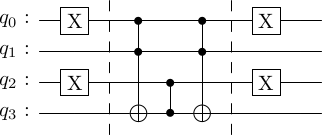
\includegraphics[width=9cm,height=10cm,keepaspectratio]{3-qubit-010.png}}
	\caption{Oracle design for 3-qubit Grover’s algorithm with 010 as solution.}
	\label{fig:3-qubit}
\end{figure}

\begin{figure}[htbp]
	\centerline{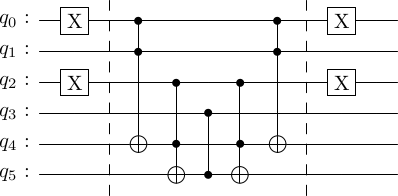
\includegraphics[width=9cm,height=10cm,keepaspectratio]{4-qubit-0101.png}}
	\caption{Oracle design for 4-qubit Grover's algorithm with01011 as solution.}
	\label{fig:4-qubit}
\end{figure}

\begin{figure}[htbp]
	\centerline{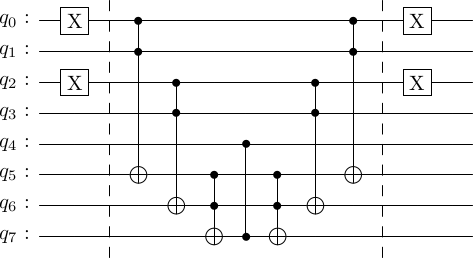
\includegraphics[width=9cm,height=10cm,keepaspectratio]{5-qubit-01011.png}}
	\caption{Oracle design for 5-qubit Grover's algorithm with 01011 as solution.}
	\label{fig:5-qubit}
\end{figure}

\subsection{Diffusion operator}
The diffusion operation can be realised through the sequence: \textbf{HX+$\textbf{C}^{\textbf{n-1}}\textbf{Z}$+XH}. In this scenario, H symbolises
the Hadamard gate, X represents the Pauli-X gate and $C^{n-1}Z$ is a controlled Z gate with n-1 control qubits. This sequence effectively flips the amplitudes around their
mean value.

\begin{figure}[htbp]
	\centerline{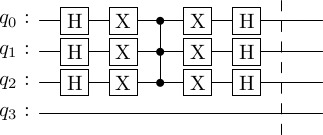
\includegraphics[width=9cm,height=10cm,keepaspectratio]{3-qubit-diff.png}}
	\caption{Diffusion operator design for 3-qubit Grover’s algorithm}
	\label{3diff}
\end{figure}

\section{Results}
3-qubit, 4-qubit and 5-qubit Grover circuits are simulated using AerSimulator from Qiskit. In addition to that 3-qubit Grover's algorithm is implemented using phase oracles on ibm\_kyiv quantum computer.
% TODO ! ADD reference
\subsection{Simulation Results}
Simulation results for 3-qubit, 4-qubit and 5-qubit Grover
search algorithm are shown in Fig \ref{fig:3_qubit}, Fig \ref{fig:4_qubit} and Fig \ref{fig:5_qubit} respectively. For 3-qubit case when searching for x=101, the algorithm yielded a success probability of 0.944. Similarly for 4 and 5 qubit cases the algorithm yielded a success probability of 0.965 and 0.999 when searching for x=1011 and x=01011. In Qiskit qubits are indexed in reverse order compared to the standard physical convention. That is why for 4-qubit and 5-qubit cases the algorithm finds \textbf{1101} and \textbf{01011} with high probability.

\begin{figure}[htbp]
	\centerline{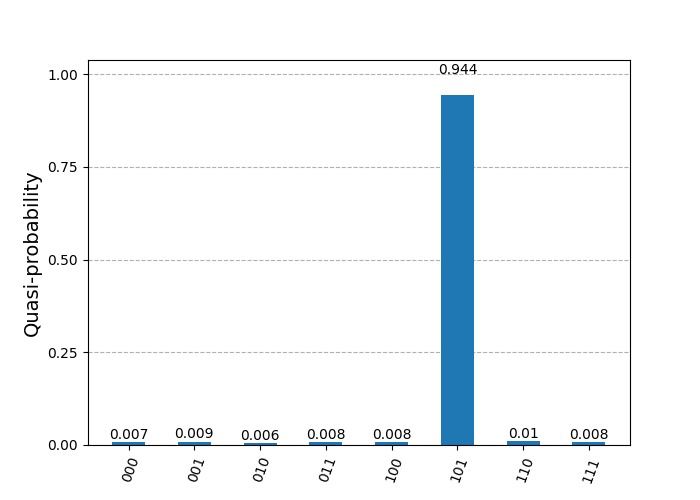
\includegraphics[width=9cm,height=10cm,keepaspectratio]{3_qubit.png}}
	\caption{Results obtained when 3-qubit Grover's algorithm using oracle from Fig \ref{fig:3-qubit}}
	\label{fig:3_qubit}
\end{figure}

\begin{figure}[htbp]
	\centerline{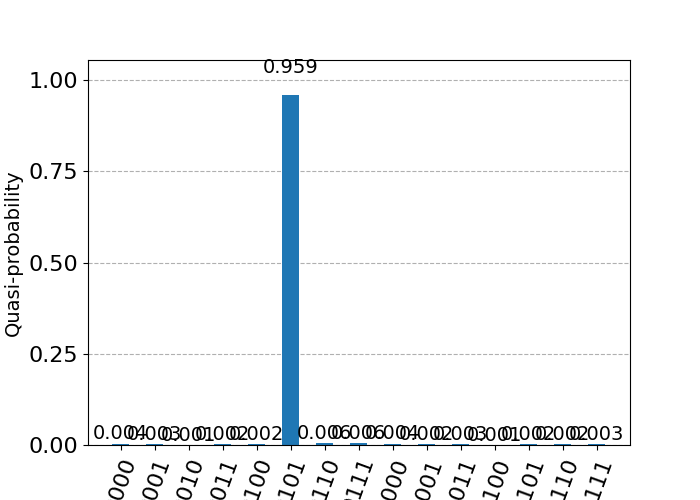
\includegraphics[width=9cm,height=10cm,keepaspectratio]{4_qubit.png}}
	\caption{Results obtained when 4-qubit Grover's algorithm using oracle from Fig \ref{fig:4-qubit}}
	\label{fig:4_qubit}
\end{figure}


\begin{figure}[htbp]
	\centerline{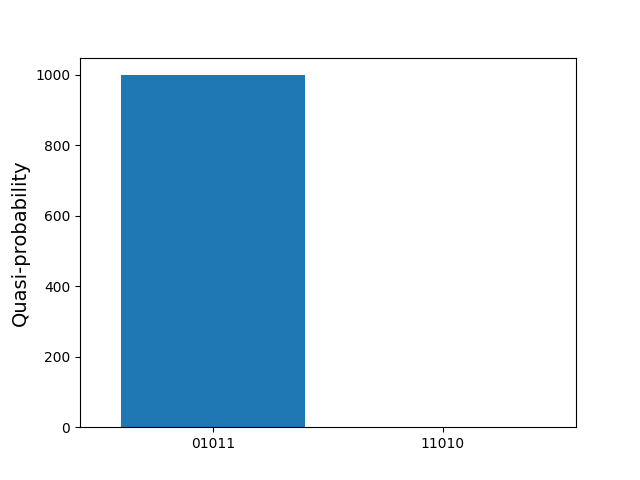
\includegraphics[width=9cm,height=10cm,keepaspectratio]{5_qubit.png}}
	\caption{Results obtained when 5-qubit Grover's algorithm using oracle from Fig \ref{fig:5-qubit}}
	\label{fig:5_qubit}
\end{figure}

\subsection{Experimental Results}
For every possible value of x (with 3 classical bits), a 3-qubit Grover circuit is constructed with phase oracle and the diffusion operator discussed above. The circuits are then transpiled and run on ibm\_kyiv quantum computer.
The circuits are run for 1024 times and the success probabilities are plotted against the value of x we are searching in Fig \ref{fig:ibm_kyiv_results}. In all the cases we observe that the success probability is more than 0.5.
\begin{figure}[htbp]
	\centerline{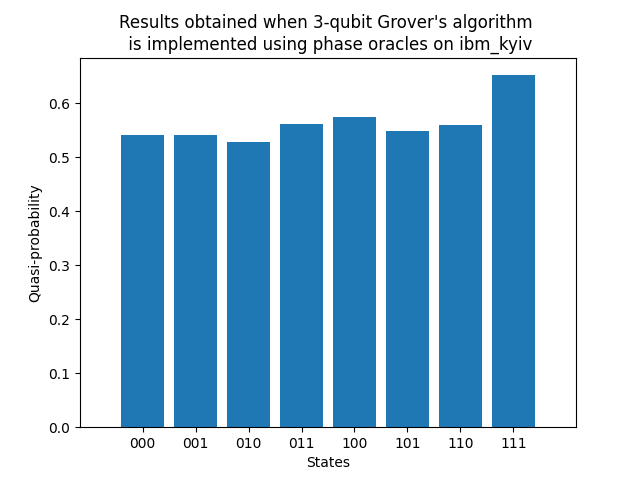
\includegraphics[width=9cm,height=10cm,keepaspectratio]{ibm_kyiv_phase_oracles.png}}
	\caption{Results obtained when 3-qubit Grover's algorithm is implemented using phase oracles on ibm\_kyiv}
	\label{fig:ibm_kyiv_results}
\end{figure}

\section{CONCLUSION}
In summary, quantum computing presents an intriguing
pathway for addressing intricate problems that surpass the capabilities of classical computers. In contrast to classical
search algorithms, which require O(N) operations for N
items, Grover's algorithm achieves this task in approximately
O($\sqrt{N} $) operations. Experimental results for Grover's algorithm on 3-qubit cases consistently yielded success probabilities exceeding 0.5, indicating the algorithm's effectiveness in practical applications.
Subsequently,
using this 5-qubit setup as a benchmark, the algorithm will
be extended to n-qubits.


\begin{thebibliography}{00}
	% TODO ? How to add a link as a reference
	\bibitem{b0} What is quantum computing?  https://www.ibm.com/topics/quantum-computing

	\bibitem{b1}  L. K. Grover, “A fast quantum mechanical algorithm for database search,” arXiv:quant-ph/9605043, Nov. 1996.

	\bibitem{b2} A. Mandviwalla, K. Ohshiro, and B. Ji, “Implementing Grover’s Algorithm on the IBM Quantum Computers.”

	\bibitem{b3} Figgatt, C., Maslov, D., Landsman, K.A. et al. Complete 3-Qubit Grover search on a programmable quantum computer. Nat Commun 8, 1918 (2017). https://doi.org/10.1038/s41467-017-01904-7

	\bibitem{b8}  C. P. Williams, “Introduction,” Texts in Computer Science, pp. 3–49,
	2011.

	\bibitem{b14}  T. D. Ladd, F. Jelezko, R. Laflamme, Y. Nakamura, C. Monroe, and
	J. L. O’Brien, “Quantum computers,” Nature, vol. 464, no. 7285, pp.
	45–53, Mar. 2010.

	\bibitem{b20} “Quantum Computing: Fundamentals, Implementations and Applications” — IEEE Journals Magazine — IEEE Xplore, ieeexplore.ieee.org.

	\bibitem{b4} D. P. DiVincenzo, “The Physical Implementation of Quantum Computation,” Fortschritte der Physik, vol. 48, no. 9–11, pp. 771–783, Sep.
	2000.
	\bibitem{b5}  D. Bacon and W. van Dam, “Recent progress in quantum algorithms,”
	Communications of the ACM, vol. 53, no. 2, pp. 84–93, Feb. 2010.

	\bibitem{b6}  N. C¸elik and ¨ O. Bing¨ ol, “Analysis of Grover’s quantum search algorithm
	on a classical computer: Identifying opportunities for improvement,”
	Sigma Journal of Engineering and Natural Sciences, vol. 42, no. 6, 2024.

	\bibitem{b7} “Learn Quantum Computing with Python and IBM Quantum Experience: A hands-on introduction to quantum computing and writing your own quantum programs with Python- Robert Loredo- Libro in linguainglese- Packt Publishing Limited- — IBS,” www.ibs.it.



	\bibitem{b9} A. J. et al., “Quantum Algorithm Implementations for Beginners,” arXiv:1804.03719 [quant-ph], Mar. 2020.

	\bibitem{b10}  “Quantum Game Simulator, Using the Circuit Model of Quantum — IEEE Conference Publication — IEEE Xplore,” ieeexplore.ieee.org.

	\bibitem{b11}  C. B. Pronin and A. V. Ostroukh, “Developing Mathematical Oracle
	Functions for Grover Quantum Search Algorithm,” arXiv.org, Sep. 03,
	2021.

	\bibitem{b12} R. L. Singleton Jr, M. L. Rogers, and D. L. Ostby, “Grover’s Algorithm
	with Diffusion and Amplitude Steering,” arXiv.org, Oct. 21, 2021.

	\bibitem{b13}  D. J. Shepherd, “On the Role of Hadamard Gates in Quantum Circuits,”
	Quantum Information Processing, vol. 5, no. 3, pp. 161–177, May 2006.



	\bibitem{b15}  D. Reddy Vemula, D. Konar, S. Satheesan, M. Kalidasu, and A. Cangi,
	“A Scalable 5,6-Qubit Grover’s Quantum Search Algorithm.”.
\end{thebibliography}

\end{document}
